% Compile with: xelatex presentation.tex   (or lualatex)
% metropolis uses the Fira Sans font, which needs XeLaTeX/LuaLaTeX.
\documentclass[aspectratio=169,11pt,c]{beamer}

\usetheme{metropolis}
\usepackage{booktabs}
\usepackage{amsmath}
\usepackage{tikz}
\usepackage{pgfplots}
\pgfplotsset{compat=1.16}
\usetikzlibrary{positioning,arrows.meta,calc,patterns}

% ---------- icon helpers for the Benefit-Rule flow chart (pure TikZ, no extra packages) ----------
\tikzset{ico/.style={line width=0.8pt,white,line cap=round,line join=round}}
\newcommand{\iconbase}[3]{% #1 centre, #2 colour, #3 drawing
 \begin{scope}[shift={#1}]
  \fill[#2] (0,0) circle (0.36cm);
  \begin{scope}[ico,scale=0.9]#3\end{scope}
 \end{scope}}
\newcommand{\iconInbox}[2]{\iconbase{#1}{#2}{%
 \draw (0,0.2)--(0,-0.07); \draw (-0.1,0.03)--(0,-0.07)--(0.1,0.03);
 \draw (-0.2,-0.04)--(-0.2,-0.17)--(0.2,-0.17)--(0.2,-0.04);}}
\newcommand{\iconBars}[2]{\iconbase{#1}{#2}{%
 \fill[white] (-0.2,-0.17) rectangle (-0.09,0.0);
 \fill[white] (-0.04,-0.17) rectangle (0.07,0.1);
 \fill[white] (0.12,-0.17) rectangle (0.23,0.2);}}
\newcommand{\iconClock}[2]{\iconbase{#1}{#2}{%
 \draw (0,0) circle (0.2); \draw (0,0)--(0,0.12); \draw (0,0)--(0.09,-0.05);}}
\newcommand{\iconScale}[2]{\iconbase{#1}{#2}{%
 \draw (0,0.2)--(0,-0.17); \draw (-0.1,-0.17)--(0.1,-0.17);
 \draw (-0.22,0.12)--(0.22,0.12);
 \draw (-0.22,0.12)--(-0.31,-0.05)--(-0.13,-0.05)--cycle;
 \draw (0.22,0.12)--(0.13,-0.05)--(0.31,-0.05)--cycle;}}
\newcommand{\iconCheck}[2]{\iconbase{#1}{#2}{%
 \draw[line width=1.3pt] (-0.15,0)--(-0.04,-0.12)--(0.17,0.13);}}
\newcommand{\iconLock}[2]{\iconbase{#1}{#2}{%
 \fill[white] (-0.16,-0.18) rectangle (0.16,0.0);
 \draw (-0.09,0.0)--(-0.09,0.07) .. controls (-0.09,0.22) and (0.09,0.22) .. (0.09,0.07)--(0.09,0.0);}}
% one box of the flow chart: icon circle on the left, centred text on the right
\newcommand{\flowbox}[6]{% #1 y, #2 height, #3 fill, #4 icon macro, #5 icon colour, #6 text
 \draw[rounded corners=3pt,fill=#3,draw=black!45,line width=0.4pt] (-4.1,#1-#2/2) rectangle (4.1,#1+#2/2);
 #4{(-3.55,#1)}{#5}
 \node[text width=6.2cm,align=center,inner sep=2pt] at (0.45,#1) {#6};}

\pgfplotsset{reportaxis/.style={tick label style={font=\scriptsize},label style={font=\small},
 legend style={font=\scriptsize,draw=none},grid=major,grid style={gray!20},axis line style={black!70}}}

% Colours used in the diagrams
\definecolor{compc}{RGB}{70,130,200}
\definecolor{commc}{RGB}{240,140,40}
\definecolor{waitc}{RGB}{170,170,170}

\title{Cost-Aware Communication Scheduling\\for Distributed Deep Learning}
\subtitle{When is a phase shift worth its pause?}
\author{Daksh Agarwal (230101123) \and Aditya Shukla (230101115)}
\institute{BTP-1 Project Presentation}
\date{}

% segment helper: \seg{x1}{x2}{y}{colour}  (times in ms)
\newcommand{\seg}[4]{\fill[#4] (#1*\sc,#3) rectangle (#2*\sc,#3+0.45);}

\metroset{block=fill}
\setbeamercolor{block title}{bg=compc!85!black,fg=white}
\setbeamercolor{block body}{bg=compc!15,fg=black}
\setbeamercolor{block title alerted}{bg=commc!90!black,fg=white}
\setbeamercolor{block body alerted}{bg=commc!15,fg=black}
\setbeamercolor{block title example}{bg=green!45!black,fg=white}
\setbeamercolor{block body example}{bg=green!12,fg=black}

\makeatletter
\setbeamertemplate{title page}{%
  \begin{minipage}[b][\textheight]{\textwidth}
    \ifx\inserttitlegraphic\@empty\else\usebeamertemplate*{title graphic}\fi
    \vfill%
    \ifx\inserttitle\@empty\else\usebeamertemplate*{title}\fi
    \ifx\insertsubtitle\@empty\else\usebeamertemplate*{subtitle}\fi
    \usebeamertemplate*{title separator}
    \ifx\beamer@shortauthor\@empty\else\usebeamertemplate*{author}\fi
    \ifx\insertdate\@empty\else\usebeamertemplate*{date}\fi
    \ifx\insertinstitute\@empty\else\usebeamertemplate*{institute}\fi
    \vfill
    \vspace*{5mm}
  \end{minipage}
}
\setbeamertemplate{progress bar in section page}{
  \setlength{\metropolis@progressonsectionpage}{%
    \textwidth * \ratio{\insertsectionnumber pt}{8pt}%
  }%
  \begin{tikzpicture}
    \fill[bg] (0,0) rectangle (\textwidth, \metropolis@progressonsectionpage@linewidth);
    \fill[fg] (0,0) rectangle (\metropolis@progressonsectionpage, \metropolis@progressonsectionpage@linewidth);
  \end{tikzpicture}%
}
\makeatother

\setbeamercovered{transparent=25}

\begin{document}

\maketitle

% ------------------------------------------------------------
% ============================================================
\section{Motivation}

\begin{frame}{Communication is the bottleneck, and two problems are overlooked}
  \begin{itemize}[<+->]\small
    \item GPU speed has outpaced network bandwidth. When distributed jobs share a cluster, their periodic \alert{communication bursts collide}.
    \item Reactive controls like DCQCN act only after network buffers fill. In contrast, application-aware schedulers like Cassini \alert{time-shift} jobs so bursts interleave peacefully.
  \end{itemize}
  \vspace{0.3em}
  \begin{columns}[T]
    \begin{column}{0.48\textwidth}
      \begin{alertblock}<+->{1. Shifts are not free}
        \scriptsize Shifting a job forces its GPUs to wait idle until the next slot arrives. For short jobs, this pause often costs more time than the network collision itself.
      \end{alertblock}
    \end{column}
    \begin{column}{0.48\textwidth}
      \begin{block}<+->{2. LCM explosion}
        \scriptsize Finding the exact repeat cycle requires computing the least common multiple of all job periods, which explodes into gigabytes of memory. Online schedulers truncate this to 600\,ms, but whether that degrades quality remained unknown.
      \end{block}
    \end{column}
  \end{columns}
\end{frame}

\begin{frame}{Research questions and contributions}
  \begin{enumerate}[<+->]
    \item When does a phase shift save enough contention delay to justify its pause?
    \item Does scoring traffic over a short window degrade schedule quality?
  \end{enumerate}
  \vspace{0.8em}
  \textbf{Contributions}
  \begin{itemize}[<+->]
    \item The \alert{Benefit Rule}, which cuts mean completion time by 9.30\% on short jobs by evaluating whether a shift is profitable.
    \item Robustness analysis showing the rule remains effective even when remaining-work estimates are off by up to 50\%.
    \item The first systematic study of LCM explosion, demonstrating that a 600\,ms window achieves 99.9\% of full-cycle schedule quality.
  \end{itemize}
\end{frame}

% ============================================================
\section{Background}

\begin{frame}{Time shifting: a simple example}
  Two identical jobs share a link with 60\,ms of compute and 40\,ms of communication per iteration.
  \vspace{0.1em}

  \centering
  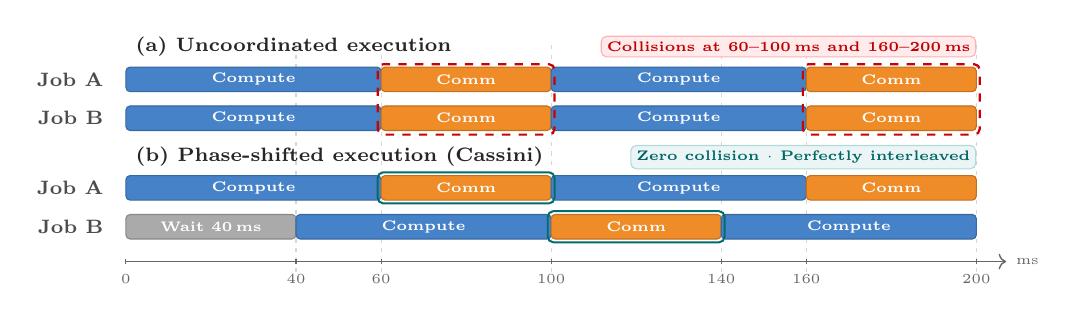
\begin{tikzpicture}[x=0.054cm, y=0.52cm]
    % --- Dotted vertical guidelines ---
    \foreach \t in {40,60,100,140,160,200} {
      \draw[dash pattern=on 1.5pt off 2pt, black!16, line width=0.4pt] (\t, -0.25) -- (\t, 5.35);
    }

    % ================= Case (a): Uncoordinated =================
    \node[anchor=west, font=\scriptsize\bfseries, text=black!85] at (0, 5.25) {(a) Uncoordinated execution};
    \node[anchor=east, font=\tiny\bfseries, text=red!75!black, fill=red!8, draw=red!30, rounded corners=2pt, inner sep=2pt] at (200, 5.25) {Collisions at 60--100\,ms and 160--200\,ms};

    % Job A
    \node[anchor=east, font=\scriptsize\bfseries, text=black!70] at (-3, 4.45) {Job A};
    \draw[fill=compc, draw=compc!80!black, rounded corners=1.5pt] (0, 4.15) rectangle (60, 4.75) node[pos=0.5, font=\tiny\bfseries\color{white}] {Compute};
    \draw[fill=commc, draw=commc!80!black, rounded corners=1.5pt] (60, 4.15) rectangle (100, 4.75) node[pos=0.5, font=\tiny\bfseries\color{white}] {Comm};
    \draw[fill=compc, draw=compc!80!black, rounded corners=1.5pt] (100, 4.15) rectangle (160, 4.75) node[pos=0.5, font=\tiny\bfseries\color{white}] {Compute};
    \draw[fill=commc, draw=commc!80!black, rounded corners=1.5pt] (160, 4.15) rectangle (200, 4.75) node[pos=0.5, font=\tiny\bfseries\color{white}] {Comm};

    % Job B
    \node[anchor=east, font=\scriptsize\bfseries, text=black!70] at (-3, 3.5) {Job B};
    \draw[fill=compc, draw=compc!80!black, rounded corners=1.5pt] (0, 3.2) rectangle (60, 3.8) node[pos=0.5, font=\tiny\bfseries\color{white}] {Compute};
    \draw[fill=commc, draw=commc!80!black, rounded corners=1.5pt] (60, 3.2) rectangle (100, 3.8) node[pos=0.5, font=\tiny\bfseries\color{white}] {Comm};
    \draw[fill=compc, draw=compc!80!black, rounded corners=1.5pt] (100, 3.2) rectangle (160, 3.8) node[pos=0.5, font=\tiny\bfseries\color{white}] {Compute};
    \draw[fill=commc, draw=commc!80!black, rounded corners=1.5pt] (160, 3.2) rectangle (200, 3.8) node[pos=0.5, font=\tiny\bfseries\color{white}] {Comm};

    % Red collision highlights behind/around the comm blocks
    \draw[red!80!black, dashed, line width=0.8pt, rounded corners=2pt] (59.2, 3.10) rectangle (100.8, 4.82);
    \draw[red!80!black, dashed, line width=0.8pt, rounded corners=2pt] (159.2, 3.10) rectangle (200.8, 4.82);

    % ================= Case (b): Time-shifted =================
    \node[anchor=west, font=\scriptsize\bfseries, text=black!85] at (0, 2.55) {(b) Phase-shifted execution (Cassini)};
    \node[anchor=east, font=\tiny\bfseries, text=teal!80!black, fill=teal!8, draw=teal!30, rounded corners=2pt, inner sep=2pt] at (200, 2.55) {Zero collision $\cdot$ Perfectly interleaved};

    % Job A
    \node[anchor=east, font=\scriptsize\bfseries, text=black!70] at (-3, 1.8) {Job A};
    \draw[fill=compc, draw=compc!80!black, rounded corners=1.5pt] (0, 1.5) rectangle (60, 2.1) node[pos=0.5, font=\tiny\bfseries\color{white}] {Compute};
    \draw[fill=commc, draw=commc!80!black, rounded corners=1.5pt] (60, 1.5) rectangle (100, 2.1) node[pos=0.5, font=\tiny\bfseries\color{white}] {Comm};
    \draw[fill=compc, draw=compc!80!black, rounded corners=1.5pt] (100, 1.5) rectangle (160, 2.1) node[pos=0.5, font=\tiny\bfseries\color{white}] {Compute};
    \draw[fill=commc, draw=commc!80!black, rounded corners=1.5pt] (160, 1.5) rectangle (200, 2.1) node[pos=0.5, font=\tiny\bfseries\color{white}] {Comm};

    % Job B
    \node[anchor=east, font=\scriptsize\bfseries, text=black!70] at (-3, 0.85) {Job B};
    \draw[fill=waitc, draw=waitc!80!black, rounded corners=1.5pt] (0, 0.55) rectangle (40, 1.15) node[pos=0.5, font=\tiny\bfseries\color{white}] {Wait 40\,ms};
    \draw[fill=compc, draw=compc!80!black, rounded corners=1.5pt] (40, 0.55) rectangle (100, 1.15) node[pos=0.5, font=\tiny\bfseries\color{white}] {Compute};
    \draw[fill=commc, draw=commc!80!black, rounded corners=1.5pt] (100, 0.55) rectangle (140, 1.15) node[pos=0.5, font=\tiny\bfseries\color{white}] {Comm};
    \draw[fill=compc, draw=compc!80!black, rounded corners=1.5pt] (140, 0.55) rectangle (200, 1.15) node[pos=0.5, font=\tiny\bfseries\color{white}] {Compute};

    % Green highlight around the interleaved communication
    \draw[teal!85!black, line width=0.7pt, rounded corners=2pt] (59.2, 1.42) rectangle (100.8, 2.18);
    \draw[teal!85!black, line width=0.7pt, rounded corners=2pt] (99.2, 0.47) rectangle (140.8, 1.23);

    % ================= Time axis =================
    \draw[->, black!60, line width=0.5pt] (0, 0) -- (207, 0) node[right, font=\tiny] {ms};
    \foreach \x in {0, 40, 60, 100, 140, 160, 200} {
      \draw[black!60] (\x, 0.07) -- (\x, -0.07) node[below, font=\tiny] {\x};
    }
  \end{tikzpicture}

  \vspace{-0.2em}
  \begin{alertblock}<+->{The central trade-off}
    Shifting Job B eliminates collisions, but introduces a 40\,ms idle pause that must be justified by future congestion savings.
  \end{alertblock}
\end{frame}

\begin{frame}{Compatibility and affinity graphs}
  \begin{columns}[c]
    \begin{column}{0.44\textwidth}
      \footnotesize
      \begin{itemize}[<+->]
        \item A \textbf{compatibility score} of 1.0 represents zero contention when job bursts are mapped onto a shared timeline.
        \item An \textbf{affinity graph} connects jobs (circles) to network links (squares), with edge labels representing required phase shifts.
        \item \textbf{Tree topology.} Breadth-first search from a root job assigns consistent start offsets to all jobs without conflicts.
        \item \textbf{Cycle topology.} Conflicting offset requirements across shared links (such as $40 \neq 55$\,ms) force the scheduler to reject the placement.
      \end{itemize}
    \end{column}
    \begin{column}{0.54\textwidth}
      \centering
\resizebox{\textwidth}{!}{%
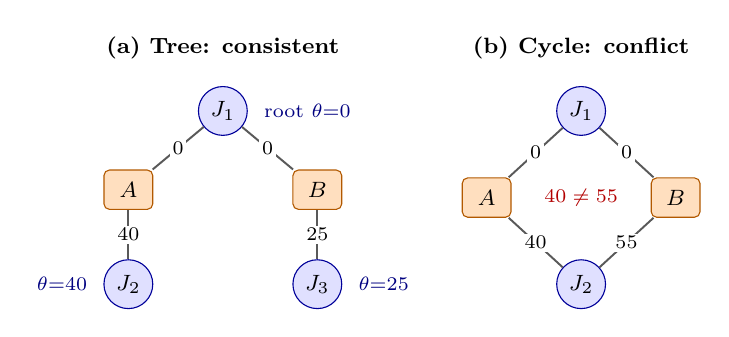
\begin{tikzpicture}[font=\footnotesize,
 job/.style={circle,draw=blue!60!black,fill=blue!12,minimum size=0.62cm,inner sep=0pt},
 lnk/.style={rectangle,rounded corners=2pt,draw=orange!70!black,fill=orange!25,minimum width=0.62cm,minimum height=0.5cm,inner sep=0pt},
 ed/.style={draw=black!65,line width=0.7pt},
 w/.style={fill=white,inner sep=1pt,font=\scriptsize}]
% ---------- (a) acyclic ----------
\begin{scope}[shift={(0,0)}]
 \node[font=\footnotesize\bfseries] at (1.95,3.35) {(a) Tree: consistent};
 \node[job] (j1) at (1.95,2.55) {$J_1$};
 \node[lnk] (a)  at (0.75,1.55) {$A$};
 \node[lnk] (b)  at (3.15,1.55) {$B$};
 \node[job] (j2) at (0.75,0.35) {$J_2$};
 \node[job] (j3) at (3.15,0.35) {$J_3$};
 \draw[ed] (j1)--node[w]{0}(a); \draw[ed] (j1)--node[w]{0}(b);
 \draw[ed] (a)--node[w,pos=0.5]{40}(j2); \draw[ed] (b)--node[w,pos=0.5]{25}(j3);
 \node[anchor=east,font=\scriptsize,text=blue!50!black] at (0.35,0.35) {$\theta{=}40$};
 \node[anchor=west,font=\scriptsize,text=blue!50!black] at (3.55,0.35) {$\theta{=}25$};
 \node[anchor=west,font=\scriptsize,text=blue!50!black] at (2.35,2.55) {root $\theta{=}0$};
\end{scope}
% ---------- (b) cycle ----------
\begin{scope}[shift={(4.55,0)}]
 \node[font=\footnotesize\bfseries] at (1.95,3.35) {(b) Cycle: conflict};
 \node[job] (k1) at (1.95,2.55) {$J_1$};
 \node[lnk] (c)  at (0.75,1.45) {$A$};
 \node[lnk] (d)  at (3.15,1.45) {$B$};
 \node[job] (k2) at (1.95,0.35) {$J_2$};
 \draw[ed] (k1)--node[w]{0}(c); \draw[ed] (k1)--node[w]{0}(d);
 \draw[ed] (c)--node[w]{40}(k2); \draw[ed] (d)--node[w]{55}(k2);
 \node[red!70!black,font=\scriptsize,align=center] at (1.95,1.45) {$40\neq 55$};
\end{scope}
\end{tikzpicture}}
    \end{column}
  \end{columns}
\end{frame}

% ============================================================
\section{System Model}

\begin{frame}{System model: link traffic and compatibility score}
  \footnotesize
  \setlength{\abovedisplayskip}{3pt}
  \setlength{\belowdisplayskip}{3pt}
  \begin{itemize}[<+->]
    \item \textbf{Periodic link traffic.} Distributed training jobs alternate between compute and communication with iteration period $T_j$. Shifting job $j$ by offset $\theta_j$ delays its periodic burst pattern $b_j(t)$. The total offered load on link $\ell$ at time $u$ sums all concurrent jobs:
    \[ B_\ell(u;\boldsymbol{\theta}) = \sum_{j \in \mathcal{J}_\ell} b_j\big((u - \theta_j) \bmod T_j\big) \]

    \item \textbf{Compatibility score.} When offered load exceeds link capacity $C_\ell$, bursts collide and queue. Over an observation window of $M$ samples ($\delta = 1$\,ms resolution, 600\,ms window), link quality penalises capacity violations:
    \[ S_\ell = 1 - \frac{1}{M C_\ell} \sum_{k=0}^{M-1} \max\big\{0,\, B_\ell(k\delta;\boldsymbol{\theta}) - C_\ell\big\} \]
  \end{itemize}
  \vspace{-0.3em}
  \begin{block}<+->{Physical meaning}
    \scriptsize $S_\ell = 1.0$ represents collision-free burst interleaving. Lower scores indicate severe link congestion and packet queuing.
  \end{block}
\end{frame}

\begin{frame}{System model: shift delay, contention and completion time}
  \footnotesize
  \setlength{\abovedisplayskip}{3pt}
  \setlength{\belowdisplayskip}{3pt}
  \begin{itemize}[<+->]
    \item \textbf{Forward phase-shift delay.} Moving job $j$ to a new offset $\theta_j'$ pauses workers until the target slot arrives. Because shifts cannot travel backwards in time, the job idles with zero training progress:
    \[ d_j = (\theta_j' - \theta_j) \bmod T_j \]

    \item \textbf{Contention penalty and completion time.} Unmitigated link contention slows iterations by penalty factor $F(S) = 1 + \lambda(1 - S)$, where $\lambda = 1.5$. For remaining work $R_j = (1 - r_j)N_jT_j$ and accumulated waiting time $w_j$ at current time $t$:
    \[ \hat c_j = t + w_j + R_j\,F(S), \qquad \mathrm{JCT}_j = c_j - a_j \]
  \end{itemize}
  \vspace{-0.3em}
  \begin{block}<+->{Greedy candidate offset search}
    \scriptsize The scheduler fixes the first job at offset 0 and searches candidate offsets in 1\,ms increments (2\,ms for three or more jobs) to find the schedule that maximizes link compatibility.
  \end{block}
\end{frame}

% ============================================================
\section{Shift Policies}

\begin{frame}{Five policies, same candidate offsets}
  All policies receive identical proposed offsets and differ only in when they accept a shift.
  \vspace{0.6em}

  \small
  \begin{tabular}{@{}lp{0.68\textwidth}@{}}
    \toprule
    \textbf{Policy} & \textbf{Decision Rule} \\
    \midrule
    Uncoordinated & Runs jobs without shifts under standard FIFO contention. \\
    Vanilla & Accepts every shift unconditionally without considering pause cost. \\
    Score Control & Accepts only if link score strictly improves, ignoring pause cost. \\
    Cooldown & Accepts only after a 100\,ms timer expires from the previous shift. \\
    \alert{Benefit Rule} & Accepts only if projected congestion savings exceed the upfront pause. \\
    \bottomrule
  \end{tabular}
\end{frame}

\begin{frame}{The Benefit Rule: evaluating shift profitability}
  \footnotesize
  \setlength{\abovedisplayskip}{2pt}
  \setlength{\belowdisplayskip}{2pt}
  \begin{itemize}[<+->]
    \item \textbf{Retaining current plan ($\widehat{L}_0$).} Jobs continue under current contention $S_0$ for estimated remaining work $\widehat{R}_j$, plus any pending wait $w_j$:
    \[ \widehat{L}_0 = \frac{1}{|\mathcal{A}|}\sum_{j \in \mathcal{A}}\big[w_j + \widehat{R}_j\,F(S_0)\big] \]

    \item \textbf{Applying candidate shift ($\widehat{L}_1$).} Jobs gain improved compatibility $S_1$, but must first pay an upfront forward idling pause $d_j$:
    \[ \widehat{L}_1 = \frac{1}{|\mathcal{A}|}\sum_{j \in \mathcal{A}}\big[w_j + d_j + \widehat{R}_j\,F(S_1)\big] \]
  \end{itemize}
  \vspace{-0.4em}
  \begin{block}<+->{Decision rule: accept shift only if $\widehat{L}_0 - \widehat{L}_1 > \varepsilon$}
    \scriptsize Accepts the shift only when projected congestion savings strictly exceed the upfront pause cost. Uses only remaining iteration counts and link scores without cluster simulation ($\varepsilon=0$\,ms in main experiments).
  \end{block}
\end{frame}

\begin{frame}{The Benefit Rule: a worked numerical example}
  \footnotesize
  \begin{itemize}[<+->]
    \item \textbf{Scenario.} Proposed shift improves link score from $S_0 = 0.6$ to $S_1 = 0.8$, reducing iteration slowdown factor $F$ from 1.6 to 1.3 (saving $0.3\,\text{ms}$ per millisecond of remaining work, $0.3\,R_j$).
    \item \textbf{Upfront cost.} Aligning to the new phase slot requires an idle pause of $d_j = 40\,\text{ms}$.
  \end{itemize}

  \vspace{0.2em}
  \begin{center}\footnotesize
  \uncover<3->{%
  \begin{tabular}{lccc}
    \toprule
    \textbf{Job Type} & \textbf{Congestion Saving} & \textbf{Upfront Pause} & \textbf{Net Benefit} \\
    \midrule
    Short job ($R_j = 100$\,ms) & $0.3 \times 100 = 30$\,ms & 40\,ms & $\mathbf{-10}$\,ms $\Rightarrow$ \alert{\textbf{Reject}} \\
    Long job ($R_j = 1000$\,ms) & $0.3 \times 1000 = 300$\,ms & 40\,ms & $\mathbf{+260}$\,ms $\Rightarrow$ \textbf{Accept} \\
    \bottomrule
  \end{tabular}%
  }
  \end{center}

  \vspace{0.2em}
  \begin{alertblock}<4->{The core economic insight}
    \scriptsize \textbf{Remaining lifespan decides whether a shift pays off.} Long jobs run long enough to amortize the pause, whereas short jobs finish before recouping the delay. Unconditional shifting (vanilla) harms short jobs.
  \end{alertblock}
\end{frame}

\begin{frame}{Benefit Rule: decision flow}
  \begin{columns}[c]
    \begin{column}{0.5\textwidth}
      \centering
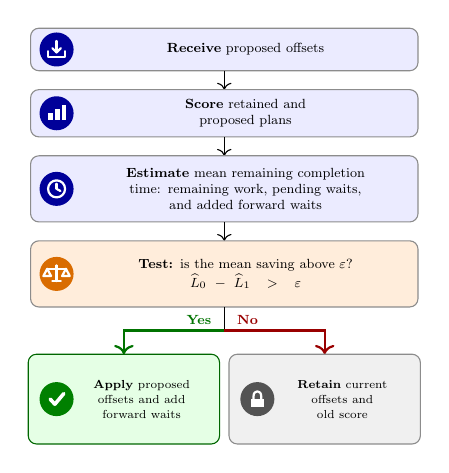
\begin{tikzpicture}[font=\footnotesize,scale=0.60,transform shape]
% Box 1: y = 4.8, h = 0.9  -> top = 5.25, bot = 4.35
\flowbox{4.8}{0.9}{blue!8}{\iconInbox}{blue!60!black}{\textbf{Receive} proposed offsets}

% Arrow 1 -> 2
\draw[->] (0, 4.35) -- (0, 3.95);

% Box 2: y = 3.45, h = 1.0 -> top = 3.95, bot = 2.95
\flowbox{3.45}{1.0}{blue!8}{\iconBars}{blue!60!black}{\textbf{Score} retained and\\ proposed plans}

% Arrow 2 -> 3
\draw[->] (0, 2.95) -- (0, 2.55);

% Box 3: y = 1.85, h = 1.4 -> top = 2.55, bot = 1.15
\flowbox{1.85}{1.4}{blue!8}{\iconClock}{blue!60!black}{\textbf{Estimate} mean remaining completion\\ time: remaining work, pending waits,\\ and added forward waits}

% Arrow 3 -> 4
\draw[->] (0, 1.15) -- (0, 0.75);

% Box 4: y = 0.05, h = 1.4 -> top = 0.75, bot = -0.65
\flowbox{0.05}{1.4}{orange!14}{\iconScale}{orange!85!black}{\textbf{Test:} is the mean saving above $\varepsilon$?\\[2pt] $\widehat{L}_0-\widehat{L}_1>\varepsilon$}

% Decision arrows
\draw (0, -0.65) -- (0, -1.15);
\draw[->,green!45!black,thick] (0, -1.15) -| (-2.125, -1.65);
\draw[->,red!60!black,thick] (0, -1.15) -| (2.125, -1.65);
\node[green!45!black,font=\footnotesize\bfseries,anchor=south east] at (-0.15, -1.15) {Yes};
\node[red!60!black,font=\footnotesize\bfseries,anchor=south west] at (0.15, -1.15) {No};

% outcomes at y = -2.6, h = 1.9 (from -1.65 to -3.55)
\draw[rounded corners=3pt,fill=green!10,draw=green!40!black,line width=0.4pt] (-4.15, -3.55) rectangle (-0.1, -1.65);
\iconCheck{(-3.55, -2.6)}{green!50!black}
\node[text width=2.4cm,align=center,inner sep=0pt,font=\scriptsize] at (-1.75, -2.6) {\textbf{Apply} proposed\\[1pt]offsets and add\\[1pt]forward waits};

\draw[rounded corners=3pt,fill=gray!12,draw=black!45,line width=0.4pt] (0.1, -3.55) rectangle (4.15, -1.65);
\iconLock{(0.7, -2.6)}{gray!65!black}
\node[text width=2.4cm,align=center,inner sep=0pt,font=\scriptsize] at (2.5, -2.6) {\textbf{Retain} current\\[1pt]offsets and\\[1pt]old score};
\end{tikzpicture}
    \end{column}
    \begin{column}{0.46\textwidth}
      \small
      \begin{itemize}[<+->]
        \item The rule tests each proposal against the retained schedule, across all affected jobs.
        \item If the mean saving exceeds $\varepsilon$, the new offsets are applied and the waits are added.
        \item Otherwise the current offsets and old score are kept.
      \end{itemize}
      \begin{alertblock}<+->{Main experiments}
        With $\varepsilon=0$\,ms, any strictly profitable shift is accepted.
      \end{alertblock}
    \end{column}
  \end{columns}
\end{frame}

% ============================================================
\section{Experimental Setup}

\begin{frame}{Workloads and evaluation methodology}
  \centering\footnotesize
  \begin{tabular}{lrrll}
    \toprule
    Workload & Jobs & Links & Source & Arrival \\
    \midrule
    Generated & 50 & 16 & Synthetic & Global \\
    Sample & 60 & 16 & Illustrative trace & Global \\
    Short & 200 & 4 & Synthetic & Incremental \\
    Large & 2000 & 32 & Synthetic trace & Incremental \\
    Scale & 10000 & 32 & Synthetic trace & Incremental \\
    \bottomrule
  \end{tabular}
  \vspace{0.4em}
  \begin{itemize}[<+->]\scriptsize
    \item \textbf{Cluster setup.} 50\,Gbps links, 1\,ms sampling resolution, 600\,ms evaluation window, and penalty parameter $\lambda = 1.5$.
    \item \textbf{Workload profiles.} Short jobs run 1 to 5 iterations, reflecting hyperparameter tuning and early-stopping trials.
    \item \textbf{Primary metric.} Percentage reduction in mean completion time relative to vanilla Cassini across paired seeds.
    \item \textbf{Robustness tests.} Evaluated under estimation error from $-50\%$ to $+50\%$, and tested across seven period families.
  \end{itemize}
\end{frame}

% ============================================================
\section{Results}

\begin{frame}{Mean JCT reduction vs.\ vanilla (\%)}
  \centering
  \begin{tabular}{lrrrr}
    \toprule
    Workload & Uncoord. & Score Ctrl & Cooldown & \alert{Benefit Rule} \\
    \midrule
    Generated & $-5.15$ & 0.33 & $-0.18$ & \textbf{1.55} \\
    Sample & $-5.62$ & 0.72 & $-0.46$ & \textbf{1.98} \\
    Short & 2.28 & 5.23 & 3.97 & \textbf{9.30} \\
    Large & $-32.72$ & 0.98 & $-0.01$ & \textbf{0.98} \\
    Scale & $-45.73$ & 3.11 & $-0.003$ & \textbf{3.11} \\
    \bottomrule
  \end{tabular}

  \vspace{0.3em}
  {\scriptsize Positive values indicate speedup. On Short, per-seed gains reach 7.95\% to 10.84\%, while tail latency falls 8.04\%.}
  \begin{columns}[T]
    \begin{column}{0.48\textwidth}
      \begin{alertblock}<+->{Short jobs}\scriptsize Doing nothing beats vanilla (+2.28\%). Unconstrained 40\,ms pauses cost more time than the collisions they prevent.\end{alertblock}
    \end{column}
    \begin{column}{0.48\textwidth}
      \begin{block}<+->{Large clusters}\scriptsize Uncoordinated execution degrades performance by up to 45.7\%. The Benefit Rule matches Score Control because long jobs amortize the pause.\end{block}
    \end{column}
  \end{columns}
\end{frame}

\begin{frame}{Why it works: fewer, better shifts}
  \begin{columns}[T]
    \begin{column}{0.46\textwidth}
      \centering
      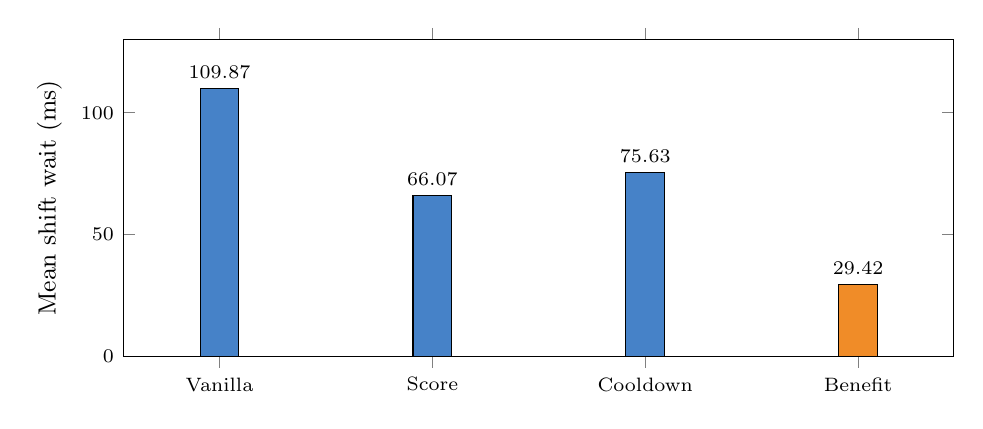
\begin{tikzpicture}
        \begin{axis}[
          ybar, width=\textwidth, height=5.6cm,
          symbolic x coords={Vanilla,Score,Cooldown,Benefit},
          xtick=data, ymin=0, ymax=130,
          ylabel={Mean shift wait (ms)},
          bar width=14pt, enlarge x limits=0.15,
          tick label style={font=\scriptsize}, ylabel style={font=\small}]
          \addplot[fill=compc, bar shift=0pt, nodes near coords, nodes near coords style={font=\scriptsize}]
            coordinates {(Vanilla,109.87) (Score,66.07) (Cooldown,75.63) (Benefit,29.42)};
          \addplot[fill=commc, bar shift=0pt] coordinates {(Benefit,29.42)};
        \end{axis}
      \end{tikzpicture}
    \end{column}
    \begin{column}{0.5\textwidth}
      \scriptsize
      On the Short workload, the Benefit Rule eliminates \alert{70\% of shift events} (falling from 480 to 144) and cuts idle wait by \alert{73\%}.
      \begin{block}<+->{Parameter sensitivity}
        Raising the minimum benefit threshold to 5\,ms produces consistent gains (up to 9.90\%), showing the rule does not require delicate tuning.
      \end{block}
      \begin{alertblock}<+->{Why static timers fail}
        Cooldown timers track wall-clock time rather than remaining work. They block profitable shifts for newly arrived long jobs and allow wasteful shifts for dying jobs.
      \end{alertblock}
    \end{column}
  \end{columns}
\end{frame}

\begin{frame}{Robustness to remaining-work estimation error}
  \begin{columns}[c]
    \begin{column}{0.6\textwidth}
      \centering
      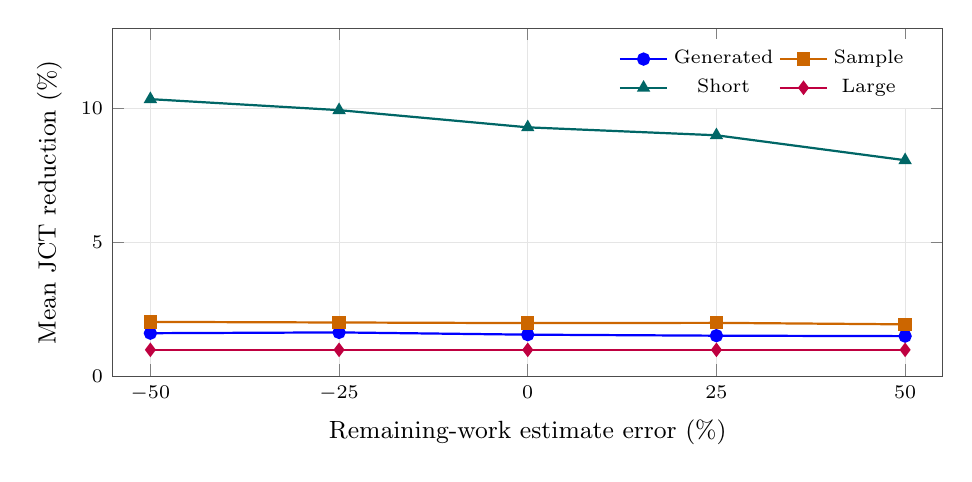
\begin{tikzpicture}
      \begin{axis}[reportaxis,width=\textwidth,height=6cm,xlabel={Remaining-work estimate error (\%)},
       ylabel={Mean JCT reduction (\%)},xmin=-55,xmax=55,ymin=0,ymax=13,
       xtick={-50,-25,0,25,50},legend columns=2,legend pos=north east]
      \addplot[blue,mark=*,thick] coordinates {(-50,1.6044) (-25,1.6335) (0,1.5495) (25,1.5113) (50,1.4945)};
      \addlegendentry{Generated}
      \addplot[orange!80!black,mark=square*,thick] coordinates {(-50,2.0262) (-25,2.0045) (0,1.9820) (25,1.9911) (50,1.9354)};
      \addlegendentry{Sample}
      \addplot[teal!80!black,mark=triangle*,thick] coordinates {(-50,10.3502) (-25,9.9391) (0,9.2969) (25,8.9999) (50,8.0674)};
      \addlegendentry{Short}
      \addplot[purple,mark=diamond*,thick] coordinates {(-50,0.9824) (-25,0.9824) (0,0.9824) (25,0.9824) (50,0.9824)};
      \addlegendentry{Large}
      \end{axis}
      \end{tikzpicture}
    \end{column}
    \begin{column}{0.38\textwidth}
      \scriptsize
      \begin{itemize}[<+->]
        \item Outperforms vanilla Cassini across all 60 paired runs, even with estimation errors up to $\pm50\%$.
        \item On short jobs, gains range from 10.35\% when underestimating to 8.07\% when overestimating remaining work.
        \item On large clusters, gains remain steady at 0.98\% across all error levels.
      \end{itemize}
      \begin{block}<+->{Intuition}
        Underestimating work makes the scheduler cautious, while overestimating makes it slightly eager. In both regimes, it reliably beats the vanilla baseline.
      \end{block}
    \end{column}
  \end{columns}
\end{frame}

% ============================================================
\section{Periodic Traffic Scoring}

\begin{frame}{Short windows and the cost of full-LCM evaluation}
  \small Jobs with periods of 100\,ms and 140\,ms repeat their combined pattern every 700\,ms. A 600\,ms window misses the burst collision occurring between 660 and 700\,ms.
  \begin{center}
  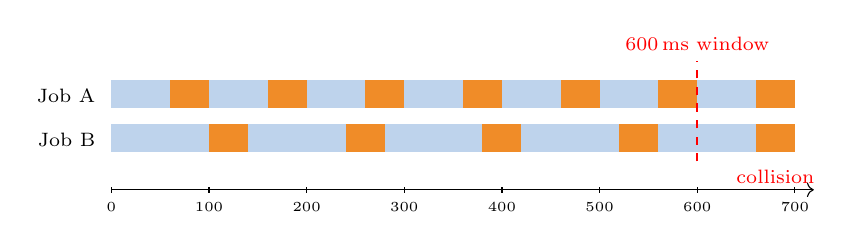
\begin{tikzpicture}[scale=0.8]
    \def\sc{0.0155}
    \node[anchor=east,font=\scriptsize] at (-0.1,1.55) {Job A};
    \fill[compc,opacity=0.35] (0,1.35) rectangle (700*\sc,1.8);
    \foreach \s in {60,160,260,360,460,560,660} { \fill[commc] (\s*\sc,1.35) rectangle ({(\s+40)*\sc},1.8); }
    \node[anchor=east,font=\scriptsize] at (-0.1,0.85) {Job B};
    \fill[compc,opacity=0.35] (0,0.65) rectangle (700*\sc,1.1);
    \foreach \s in {100,240,380,520,660} { \fill[commc] (\s*\sc,0.65) rectangle ({(\s+40)*\sc},1.1); }
    \draw[thick,dashed,red] (600*\sc,0.5) -- (600*\sc,2.1) node[above,font=\scriptsize] {600\,ms window};
    \node[red,font=\scriptsize] at (680*\sc,0.25) {collision};
    \draw[->] (0,0.05) -- (700*\sc+0.3,0.05);
    \foreach \x in {0,100,...,700} {\draw (\x*\sc,0.0)--(\x*\sc,0.1); \node[font=\tiny,below] at (\x*\sc,0) {\x};}
  \end{tikzpicture}
  \end{center}
  \vspace{-0.3em}
  \begin{block}<+->{Combinatorial explosion of full-LCM scoring}
    \scriptsize Evaluating the exact repeat cycle across prime periods requires massive computation. For four jobs with periods 101, 103, 107, and 109\,ms, the LCM exceeds 33 hours and consumes \alert{1.94\,GB} of memory. In contrast, a 600\,ms window captures 99.9\% of full-cycle schedule quality in under one millisecond.
  \end{block}
\end{frame}

\begin{frame}{Score optimism across period families}
  \begin{columns}[c]
    \begin{column}{0.6\textwidth}
      \centering
      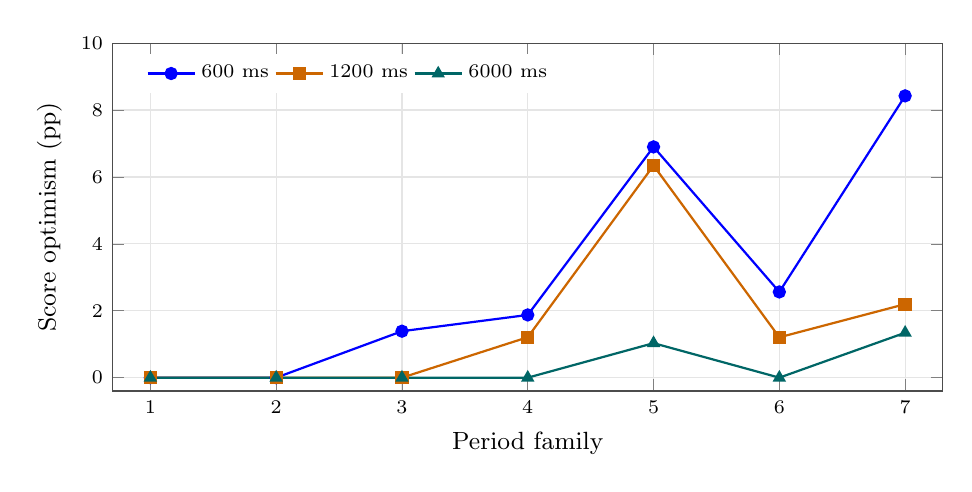
\begin{tikzpicture}
      \begin{axis}[reportaxis,width=\textwidth,height=6cm,xlabel={Period family},
       ylabel={Score optimism (pp)},xmin=0.7,xmax=7.3,ymin=-0.4,ymax=10,
       xtick={1,2,3,4,5,6,7},legend columns=3,legend pos=north west]
      \addplot[blue,mark=*,thick] coordinates {(1,0) (2,0) (3,1.3889) (4,1.8750) (5,6.8982) (6,2.5623) (7,8.4239)};
      \addlegendentry{600 ms}
      \addplot[orange!80!black,mark=square*,thick] coordinates {(1,0) (2,0) (3,0) (4,1.2094) (5,6.3427) (6,1.2063) (7,2.1976)};
      \addlegendentry{1200 ms}
      \addplot[teal!80!black,mark=triangle*,thick] coordinates {(1,0) (2,0) (3,0) (4,0) (5,1.0316) (6,0) (7,1.3429)};
      \addlegendentry{6000 ms}
      \end{axis}
      \end{tikzpicture}
    \end{column}
    \begin{column}{0.38\textwidth}
      \scriptsize
      \begin{itemize}[<+->]
        \item A 600\,ms window overestimates compatibility in 15 of 21 cases, but is exact whenever the true LCM is under 600\,ms.
        \item Optimism decreases steadily as the window expands toward the true period.
        \item Even with optimistic scores, candidate shift rankings remain accurate.
      \end{itemize}
      \vspace{-0.3em}
      \begin{alertblock}<+->{Near-optimal schedules}
        A 600\,ms window reaches within \textbf{0.08 percentage points} of an exhaustive search. Truncation yields optimistic scores, but near-optimal decisions.
      \end{alertblock}
    \end{column}
  \end{columns}
\end{frame}

% ============================================================
\section{Conclusion}

\begin{frame}{Conclusions and practical principles}
  \begin{itemize}[<+->]
    \item Phase shifting is an \alert{economic trade-off} between the upfront pause and future congestion savings.
    \item The Benefit Rule cuts average completion time by \textbf{9.30\%} and tail latency by \textbf{8.04\%} on short jobs, matches best policies on large clusters, and tolerates $\pm50\%$ estimation error.
    \item A 600\,ms evaluation window delivers 99.9\% of full-cycle schedule quality at sub-millisecond overhead.
    \item Static cooldown timers degrade performance by up to 1.72\% because they track wall-clock time rather than remaining work.
  \end{itemize}
  \vspace{-0.3em}
  \begin{block}<+->{Practical deployment}
    The rule requires only remaining iteration counts and link compatibility scores, allowing direct deployment in Slurm or Kubernetes without custom hardware.
  \end{block}
\end{frame}

\begin{frame}{Future work for BTP-2: dynamic realignment}
  \begin{itemize}[<+->]
    \item Real GPUs exhibit 2\% to 5\% step-time variance. Over hundreds of iterations, initially interleaved bursts drift and collide.
    \item Current geometric schedulers set offsets once at launch and assume perfect synchronisation throughout training.
    \item In BTP-2, we plan two mechanisms to address phase drift:
    \begin{enumerate}[<+->]
      \item \textbf{Resynchronisation checkpoints.} Periodically nudge drifting iterations back into their designated time slots.
      \item \textbf{Elastic communication cushions.} Add adaptive timing buffers to absorb variance without stalling GPUs.
    \end{enumerate}
    \item We will validate both mechanisms across cluster simulations and physical GPU testbeds.
  \end{itemize}
\end{frame}

\begin{frame}[standout]
  \fontsize{44}{50}\selectfont Thank you!\par
  \vspace{0.8em}
  \huge Questions \& Discussion
\end{frame}

\end{document}
